\section{Entropy coding}
\label{sec:entropy}

After quantization most indices are zero, and the nonzero ones are mostly $\pm1$ or $\pm2$.
WSQ codes them losslessly with a Huffman coder whose alphabet mixes coefficient values with
lengths of zero runs, in the spirit of baseline JPEG (Annex A.4 and Annex C).

\subsection{Blocks}
\label{sec:blocks}

The indices are serialized subband by subband in increasing $k$, row by row within a subband,
skipping subbands with $Q_k = 0$. The sequence is cut into \emph{blocks}, each coded with one
Huffman table. There must be at least three blocks, with breaks between subbands 18 and 19 and
between 51 and 52 (Figure~\ref{fig:subbands}); further subdivision is allowed. The breaks
separate the coarse subbands from the fine ones so that a decoder could show a low-resolution
image after the first block (\emph{progressive transmission}). Encoder number two uses exactly
three blocks, one Huffman table for block~1 (subbands 0--18) and a second, shared table for
blocks 2 and 3 (subbands 19--51 and 52--59). Zero runs may cross subband boundaries within a
block.

\subsection{The symbol alphabet}

Table~\ref{tab:symbols} lists the 254 symbols. Symbols 1 to 100 stand for runs of 1 to 100
zeros, and symbols 107 to 254 for the indices $-73$ to $74$, with symbol $s$ meaning the index
$s - 180$. The index 0 never appears as a value, so symbol 180 is unused: an isolated zero is a
run of length one. Anything outside these ranges is coded with an escape symbol followed by the
raw value in 8 or 16 bits, most significant bit first. Indices are signed, but the escape
carries the magnitude and the symbol carries the sign. Algorithm~\ref{alg:tokenize} turns a
block into symbols the way the NIST encoder does, which also fixes the choices the
specification leaves open (for example, a run of 300 zeros becomes one 16-bit escape rather
than several shorter runs).

\begin{table}[ht]
  \centering\small
  \begin{tabular}{@{}rl@{}}
    \toprule
    symbol $s$ & meaning\\
    \midrule
    1--100 & a run of $s$ zeros\\
    101 & escape: positive index, 8-bit magnitude follows\\
    102 & escape: negative index, 8-bit magnitude follows\\
    103 & escape: positive index, 16-bit magnitude follows\\
    104 & escape: negative index, 16-bit magnitude follows\\
    105 & escape: run of zeros, 8-bit length follows\\
    106 & escape: run of zeros, 16-bit length follows\\
    107--254 & the index $s - 180$, from $-73$ to $74$ (symbol 180 is never used)\\
    \bottomrule
  \end{tabular}
  \caption{Huffman input symbols (Table A.2 of the specification).}
  \label{tab:symbols}
\end{table}

\begin{algorithm}[ht]
  \caption{Turning a block of indices into symbols (as in the NIST encoder).}
  \label{alg:tokenize}
  \begin{algorithmic}[1]
    \Require indices $p_1, \dots, p_N$ of one block
    \Ensure symbols, each possibly followed by an extra field of $b$ raw bits
    \Procedure{EmitRun}{$n$}
      \If{$n \le 100$} emit symbol $n$
      \ElsIf{$n \le 255$} emit $105$ and $n$ in 8 bits
      \Else\ emit $106$ and $n$ in 16 bits
      \EndIf
    \EndProcedure
    \State $n \gets 0$
    \For{$i \gets 1$ \textbf{to} $N$}
      \If{$p_i = 0$}
        \State $n \gets n + 1$
        \If{$n = 65535$} \Call{EmitRun}{$n$};\ $n \gets 0$ \EndIf
      \Else
        \If{$n > 0$} \Call{EmitRun}{$n$};\ $n \gets 0$ \EndIf
        \If{$-73 \le p_i \le 74$} emit symbol $p_i + 180$
        \ElsIf{$0 < p_i \le 255$} emit $101$ and $p_i$ in 8 bits
        \ElsIf{$p_i > 255$} emit $103$ and $p_i$ in 16 bits
        \ElsIf{$-255 \le p_i < 0$} emit $102$ and $-p_i$ in 8 bits
        \Else\ emit $104$ and $-p_i$ in 16 bits
        \EndIf
      \EndIf
    \EndFor
    \If{$n > 0$} \Call{EmitRun}{$n$} \EndIf
  \end{algorithmic}
\end{algorithm}

\subsection{Huffman tables}

A Huffman table is transmitted in the compact form of JPEG: a list $\mathrm{BITS}$ of 16
counts, $\mathrm{BITS}(\ell)$ being the number of codes of length $\ell$ bits, followed by the
list $\mathrm{HUFFVAL}$ of the symbols, sorted by code length (Annex C). The codes themselves
are not transmitted: both sides derive them by the \emph{canonical} rule. Codes of the same
length are consecutive binary numbers, the first code of each length follows the last code of
the previous length, and each step to a longer length appends a zero
(Algorithm~\ref{alg:codes}, which merges Figures C.1 and C.2 of the specification).

Figure~\ref{fig:hufftree} shows an example with $\mathrm{BITS} = (0, 2, 3, 1, 0, \dots)$ and
$\mathrm{HUFFVAL} = (1, 181, 179, 2, 182, 3)$. The specification requires that the code made
only of 1-bits be left unused at every length, as JPEG does. A decoder that looks for markers
can then never mistake the 1-bit padding at the end of a segment for a code.

\begin{figure}[ht]
  \centering
  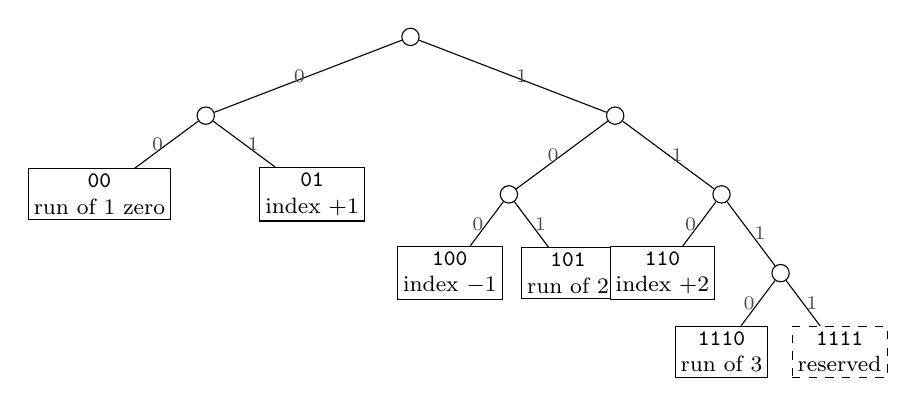
\begin{tikzpicture}[level distance=10mm,font=\footnotesize,
    inner/.style={circle,draw,fill=white,inner sep=0pt,minimum size=2.2mm},
    leaf/.style={draw,align=center,inner sep=2pt,fill=white},
    level 1/.style={sibling distance=52mm},
    level 2/.style={sibling distance=27mm},
    level 3/.style={sibling distance=15mm},
    edge from parent/.style={draw},
    bit/.style={font=\scriptsize,text=black!70,inner sep=1pt}]
  \node[inner] {}
    child {node[inner] {}
      child {node[leaf] {\texttt{00}\\run of 1 zero} edge from parent node[bit,left] {0}}
      child {node[leaf] {\texttt{01}\\index $+1$} edge from parent node[bit,right] {1}}
      edge from parent node[bit,left] {0}}
    child {node[inner] {}
      child {node[inner] {}
        child {node[leaf] {\texttt{100}\\index $-1$} edge from parent node[bit,left] {0}}
        child {node[leaf] {\texttt{101}\\run of 2} edge from parent node[bit,right] {1}}
        edge from parent node[bit,left] {0}}
      child {node[inner] {}
        child {node[leaf] {\texttt{110}\\index $+2$} edge from parent node[bit,left] {0}}
        child {node[inner] {}
          child {node[leaf] {\texttt{1110}\\run of 3} edge from parent node[bit,left] {0}}
          child {node[leaf,dashed] {\texttt{1111}\\reserved} edge from parent node[bit,right] {1}}
          edge from parent node[bit,right] {1}}
        edge from parent node[bit,right] {1}}
      edge from parent node[bit,right] {1}};
\end{tikzpicture}

  \caption{Canonical code tree for $\mathrm{BITS} = (0,2,3,1)$ and
  $\mathrm{HUFFVAL} = (1, 181, 179, 2, 182, 3)$. The all-ones word \texttt{1111} is reserved.}
  \label{fig:hufftree}
\end{figure}

\begin{algorithm}[ht]
  \caption{Canonical codes and decoding tables from BITS and HUFFVAL.}
  \label{alg:codes}
  \begin{algorithmic}[1]
    \Require $\mathrm{BITS}(1..16)$, $\mathrm{HUFFVAL}(0..n-1)$ with $n = \sum_\ell \mathrm{BITS}(\ell)$
    \Ensure $\mathrm{code}(i)$ and $\mathrm{size}(i)$ for symbol $\mathrm{HUFFVAL}(i)$; tables $\mathrm{MINCODE}$, $\mathrm{MAXCODE}$, $\mathrm{VALPTR}$
    \State $c \gets 0$;\ $i \gets 0$
    \For{$\ell \gets 1$ \textbf{to} $16$}
      \If{$\mathrm{BITS}(\ell) = 0$}
        \State $\mathrm{MAXCODE}(\ell) \gets -1$ \Comment{no code of this length}
      \Else
        \State $\mathrm{VALPTR}(\ell) \gets i$;\ $\mathrm{MINCODE}(\ell) \gets c$
        \For{$j \gets 1$ \textbf{to} $\mathrm{BITS}(\ell)$}
          \State $\mathrm{code}(i) \gets c$;\ $\mathrm{size}(i) \gets \ell$;\ $c \gets c + 1$;\ $i \gets i + 1$
        \EndFor
        \State $\mathrm{MAXCODE}(\ell) \gets c - 1$
      \EndIf
      \State $c \gets 2c$ \Comment{one bit longer}
    \EndFor
  \end{algorithmic}
\end{algorithm}

\subsection{Decoding}

Bits are packed into bytes most significant bit first (Annex C.3). A decoder reads one bit at
a time, growing a code until it falls within the range of codes of its length, and then looks
the symbol up (Algorithm~\ref{alg:huffdecode}). The symbol is expanded into indices by reading
Table~\ref{tab:symbols} backwards. Two byte-level rules apply inside an entropy-coded segment
(Annex B.1.1.5): the encoder pads the last byte with 1-bits, and after every \hex{FF} byte it
writes a \hex{00} byte (\emph{byte stuffing}), so that a marker, which is \hex{FF} followed by
a nonzero byte, can never appear by accident. The decoder drops the stuffed zeros and stops at
the first true marker, discarding any incomplete code (the padding).

\begin{algorithm}[ht]
  \caption{Decoding the indices of one block.}
  \label{alg:huffdecode}
  \begin{algorithmic}[1]
    \Require the bits of an entropy-coded segment (stuffing removed); the block's table; the number $N$ of indices still expected
    \Ensure the indices of the block, appended to the output
    \Function{DecodeSymbol}{}
      \State $c \gets$ next bit;\ $\ell \gets 1$
      \While{$c > \mathrm{MAXCODE}(\ell)$}
        \State $c \gets 2c + \text{next bit}$;\ $\ell \gets \ell + 1$
        \If{$\ell > 16$} \textbf{fail}: invalid code \EndIf
      \EndWhile
      \State \Return $\mathrm{HUFFVAL}\bigl(\mathrm{VALPTR}(\ell) + c - \mathrm{MINCODE}(\ell)\bigr)$
    \EndFunction
    \While{fewer than $N$ indices have been produced \textbf{and} bits remain}
      \State $s \gets \Call{DecodeSymbol}{}$ \Comment{stop quietly if the bits run out inside a code}
      \If{$1 \le s \le 100$} output $s$ zeros
      \ElsIf{$s = 101$ \textbf{or} $s = 103$} output the next 8 (16) bits as a positive index
      \ElsIf{$s = 102$ \textbf{or} $s = 104$} output minus the next 8 (16) bits
      \ElsIf{$s = 105$ \textbf{or} $s = 106$} output as many zeros as the next 8 (16) bits say
      \ElsIf{$107 \le s \le 254$ \textbf{and} $s \ne 180$} output $s - 180$
      \Else\ \textbf{fail}: invalid symbol
      \EndIf
    \EndWhile
  \end{algorithmic}
\end{algorithm}

A note of caution: the all-ones rule is not always honoured. Every one of the 86 WSQ files that
NIST distributes for decoder compliance testing contains a Huffman table that assigns an
all-ones code, and the NIST decoder prints a warning for each of them. A decoder should accept
such tables.

\subsection{Designing the tables}

The specification does not say how an encoder builds its tables. Encoder number two builds
them for each image from the symbol counts, using the procedure of Annex K of the JPEG standard
\cite{jpeg}, as the NIST encoder does (Algorithm~\ref{alg:hufftable}). It is ordinary Huffman
code construction with three additions: a dummy symbol with count one is added so that the
longest code, which is all ones, goes to it and is then discarded; codes longer than 16 bits
are shortened by moving leaves up the tree; and ties are broken in favour of the larger symbol
value. The length limit is not a corner case: for 59 of the 160 tables the NIST encoder builds
for its compliance images, plain Huffman construction yields codes of 17 to 20 bits. The tie
rule only matters for reproducing the NIST encoder byte for byte; with it,
Algorithm~\ref{alg:hufftable} reproduces all 160 tables exactly.

\begin{algorithm}[ht]
  \caption{An optimal table from symbol counts (JPEG Annex K.2--K.4).}
  \label{alg:hufftable}
  \begin{algorithmic}[1]
    \Require counts $F(0..255)$ of the symbols of the blocks that share the table
    \Ensure $\mathrm{BITS}(1..16)$ and $\mathrm{HUFFVAL}$
    \State $F(256) \gets 1$ \Comment{dummy symbol: reserves the all-ones code}
    \State $\mathrm{size}(v) \gets 0$ and $\mathrm{next}(v) \gets \bot$ for all $v$ \Comment{each $v$ heads a chain of merged symbols}
    \Loop
      \State $v_1 \gets$ the symbol with the smallest $F > 0$; $v_2 \gets$ the next smallest \Comment{ties: larger $v$ first}
      \If{there is no $v_2$} \textbf{break} \EndIf
      \State $F(v_1) \gets F(v_1) + F(v_2)$;\ $F(v_2) \gets 0$
      \State increment $\mathrm{size}$ of every symbol in the chains of $v_1$ and $v_2$
      \State link the chain of $v_2$ to the end of the chain of $v_1$
    \EndLoop
    \State $\mathrm{B}(\ell) \gets |\{v : \mathrm{size}(v) = \ell\}|$ for $\ell = 1..32$
    \For{$\ell \gets 32$ \textbf{down to} $17$} \Comment{limit lengths to 16 bits}
      \While{$\mathrm{B}(\ell) > 0$}
        \State $j \gets \ell - 2$; \textbf{while} $\mathrm{B}(j) = 0$: $j \gets j - 1$
        \State $\mathrm{B}(\ell) \gets \mathrm{B}(\ell) - 2$;\ $\mathrm{B}(\ell-1) \gets \mathrm{B}(\ell-1) + 1$;\ $\mathrm{B}(j+1) \gets \mathrm{B}(j+1) + 2$;\ $\mathrm{B}(j) \gets \mathrm{B}(j) - 1$
      \EndWhile
    \EndFor
    \State decrement $\mathrm{B}(\ell)$ for the largest $\ell$ with $\mathrm{B}(\ell) > 0$ \Comment{drop the dummy}
    \State $\mathrm{BITS}(\ell) \gets \mathrm{B}(\ell)$ for $\ell = 1..16$
    \State $\mathrm{HUFFVAL} \gets$ symbols $0..255$ with $\mathrm{size} > 0$, by increasing size, then increasing value
  \end{algorithmic}
\end{algorithm}
